\documentclass[12pt, letterpaper]{article}
\usepackage[utf8]{inputenc}
\usepackage[italian]{babel}
\usepackage[T1]{fontenc}
\usepackage{graphicx}
\graphicspath{}
\usepackage{listings}
\usepackage{svg}

\title{Progetto per il corso di Progetto Automatico di Sistemi Digitali}
\author{Filippo Landi}

\begin{document}
\maketitle

\begin{abstract}
Il mio progetto per il corso di \textit{Progetto Automatico di Sistemi Digitali} (\textit{PASD} in breve) consiste nello studio statistico del comportamento di un circuito \textit{multiply and accumulate} (o \textit{mac} in breve) in presenza di alcuni difetti di produzione.
\end{abstract}

\section{Introduzione al progetto}

Il progetto riguarda il collaudo dei sistemi digitali, un argomento trattato ampiamente nel corso.

Al fine di simulare i guasti del circuito userò \textit{HOPE}: un simulatore di guasto per circuiti digitali sequenziali sviluppato dall'università VirginiaTech, uno strumento di Electronic Design Automation proposto durante il corso.

HOPE è un software per le università e la ricerca, per averne una copia bisogna entrare in contatto con l'università di VirginiaTech: io non lo condividerò in questo progetto.

HOPE legge i circuiti attraverso delle descrizioni della rete (dette anche \textit{netlist}) in formato \textit{.bench}, infatti il primo punto del progetto sarà l'implementazione del circuito in questo formato.

Ho usato \textit{Python} per diversi passaggi del progetto: 
\begin{itemize}
\item Non è un linguaggio efficiente come ad esempio il linguaggio C, però mette a disposizione funzioni built-in per la manipolazione di stringhe che si sono rivelate molto comode da usare.
\item Ci sono molte librerie interessanti per Python come la libreria \textit{matplotlib} che mi ha permesso in maniera comoda di realizzare dei grafici dei dati raccolti.
\end{itemize}

I prerequisiti software quindi sono:
\begin{enumerate} 
\item \textit{Python} in versione superiore alla 3.6.
\item Il software \textit{HOPE}.
\item La libreria \textit{matplotlib} (con le varie dipendenze).
\end{enumerate}

Ho inoltre modificato gli script per renderli compatibili con la versione 2.7 di Python tranne per quanto riguarda la realizzazione automatica dei grafici: ho trovato qualche problema probabilmente perché matplotlib si è installato per la mia versione (versione 3.8.10), probabilmente creando degli ambienti virtuali si risolve ma non ho esplorato questa via.

L'esposizione del progetto seguirà questo flusso: 
\begin{enumerate}
\item Partiremo dalla descrizione del circuito da studiare in termini di porte logiche.
\item Passeremo poi ad analizzare la sua implementazione attraverso uno script Python.
\item Vedremo come usare HOPE per i nostri scopi.
\item Estrapoleremo dei dati e calcoleremo delle statistiche attraverso un altro script.
\item Infine vedremo e commenteremo i risultati con alcuni grafici.
\end{enumerate}

\section{Circuito multiply and accumulate}

Mi è stato richiesto di realizzare un circuito multiply and accumulate (mac) a 8 bit, esso è composto da un moltiplicatore con un sommatore in cascata e un registro per retroazionare le uscite in modo da accumulare i risultati.

Riporto un documento inviatomi dal professore che illustra gli schemi di un circuito di questo tipo a 4 bit.

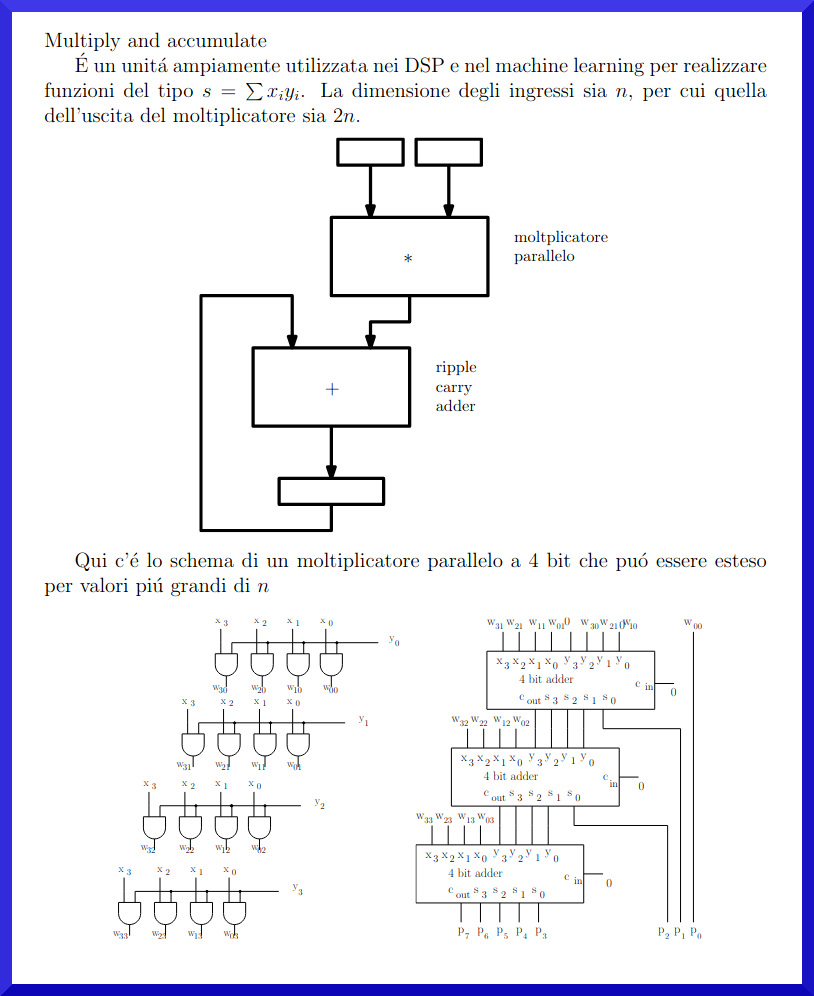
\includegraphics[width=13cm]{mac.png}

\newpage
\subsection{Moltiplicatore}
La struttura del moltiplicatore è ben illustrata nella documentazione:

\begin{itemize}
  \item Ogni segnale X è messo in AND con ogni Y, generando i segnali W.
  \item I segnali W vengono usati da degli adder strutturati su più livelli: si può notare che il numero di livelli è n-1 in quanto al primo livello vengono usati WX1 e WX0, poi i rimanenti WXY nei livelli successivi.
\end{itemize}

\subsection{Sommatore}
È un \textit{ripple carry adder} (\textit{rca} in breve) con dimensione degli ingressi 2n: un ingresso è dato dall'uscita del moltiplicatore mentre l'altra è data dalle uscite stesse del sommatore retroazionate attraverso dei flip-flop tipo D (circuito già integrato in HOPE).

\subsubsection{Ripple Carry Adder}

Usiamo dei circuiti ripple carry adder sia per la cascata di adder del moltiplicatore oltre che per il successivo sommatore.

Questi circuiti nella precedente documentazione erano illustrati a livello \textit{register transfer level} (\textit{RTL}) per ragioni di chiarezza: per l'implementazione ci serve vedere come sono fatti a livello di porte logiche.

Gli rca sono formati da una serie di adder opportunamente collegati: gli adder sono half-adder o full-adder a seconda del peso del bit.

\begin{figure}
\centering
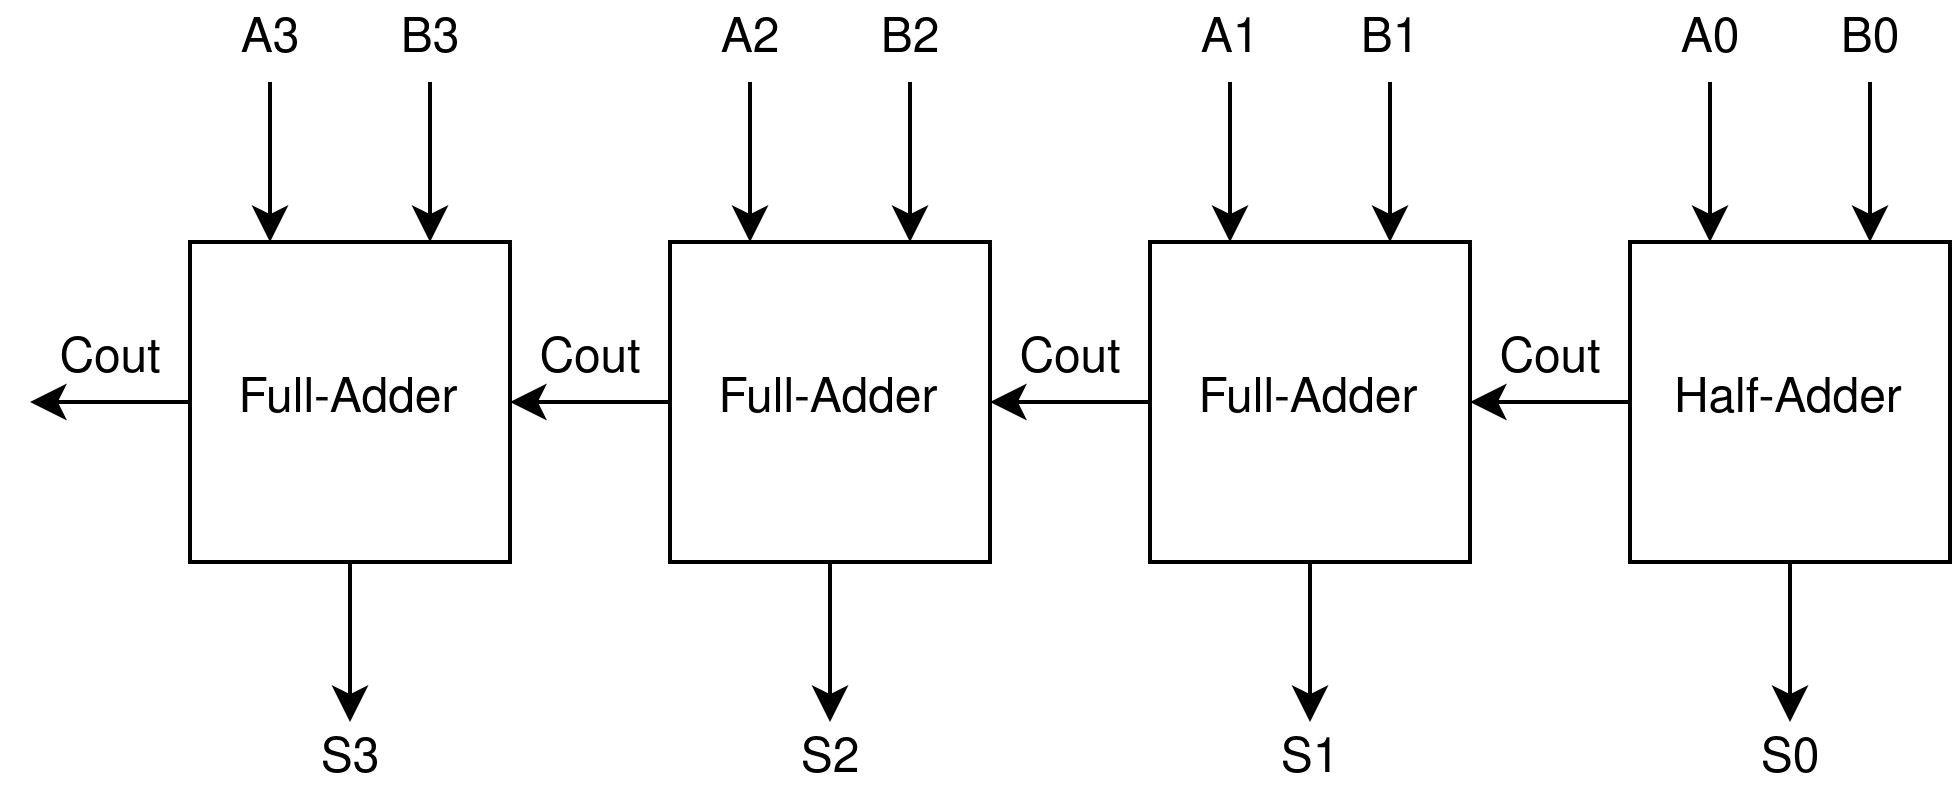
\includegraphics[width=\textwidth]{ripple_carry_adder}
\caption{Schema del ripple carry adder.}
\label{rca}
\end{figure}

\begin{figure}
\centering

\includegraphics{half_adder}
\caption{Schema dell'half-adder.}
\end{figure}

\begin{figure}
\centering
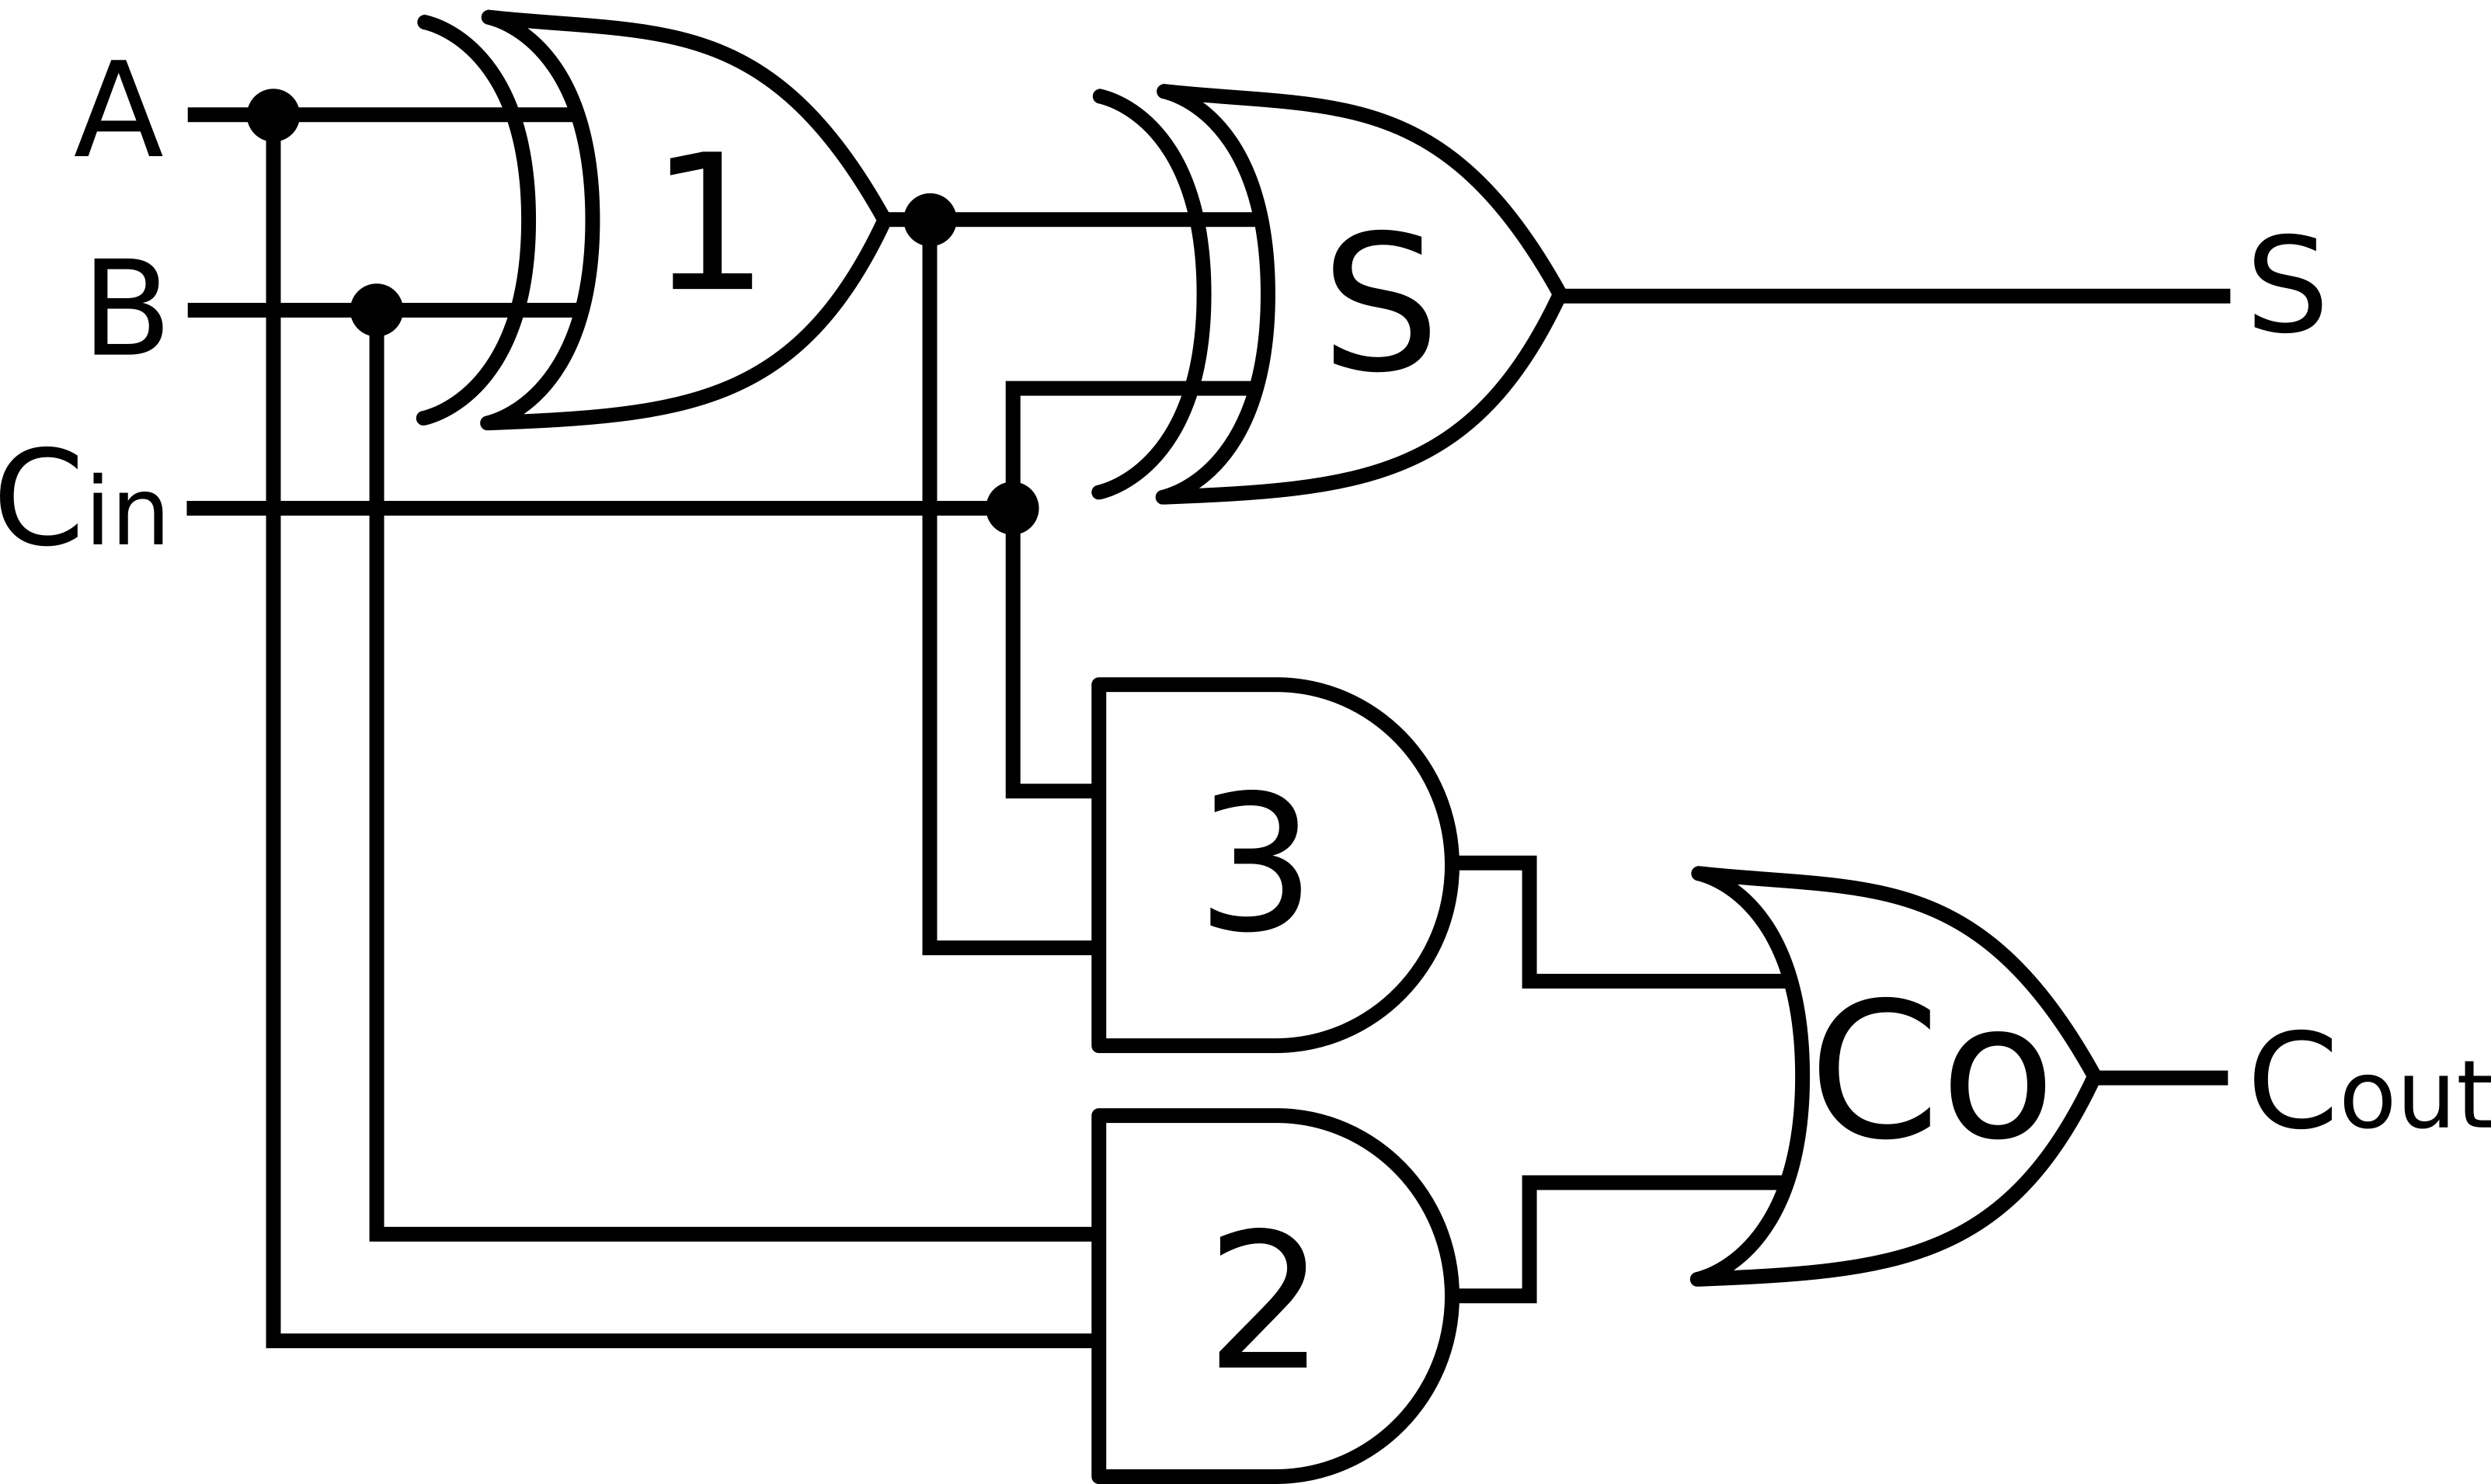
\includegraphics[width=8cm]{full_adder}
\caption{Schema del full-adder.}
\end{figure}

Si possono vedere gli schemi alla pagina \pageref{rca}.

\section{Script mac\_generator.py}

La stesura manuale del file .bench del mac ad 8 bit non mi sembrava un approccio furbo vista l'architettura piuttosto complessa da rappresentare. Probabilmente proseguire con tale metologia avrebbe portato a vari errori: sia banalmente di battitura, sia dovuti alla complessità e quindi errori nel collegamento dei vari segnali. Per questo ho pensato ad una metodologia stile \textit{divide et impera}.

In partenza ho scritto alcuni circuiti di prova per esplorare i vari adder e la prima parte del moltiplicatore.
Li trovate nella cartella \textit{circuti\_prova}: non sono fondamentali per il progetto però possono aiutare alla comprensione della metodologia usata.

Appurata la struttura dei circuiti base, ho creato uno script monolitico \textit{mac\_generator.py} che attraverso alcuni cicli e condizioni li collega in maniera consistente con gli schemi a mia disposizione.
Questo script permette di generare mac con dimensione arbitraria degli ingressi da passare come argomento.
Ad esempio per generare un mac 4 bit si può scrivere da terminale questo comando Python: 

\begin{lstlisting}
python3 mac_generator.py 4  
\end{lstlisting}

Il passo successivo sarebbe un approccio più modulare, che otterrebbe lo stesso risultato chiamando sottofunzioni per la varie parti del circuito: per i miei scopi uno script monolitico è più che sufficiente quindi mi fermo a questa versione.

Il codice è ampiamente commentato quindi consiglio di leggerlo per comprenderne il funzionamento.

L'unico punto che potrebbe essere difficoltoso è la comprensione dei vari segnali, proprio per questo un approccio manuale a mio avviso non sarebbe stato efficiente.

Descrivo la struttura dei vari segnali sperando di fare un po' di chiarezza:

\begin{itemize}

\item Gli input sono facilmente individuabili e sono X e Y seguiti dal rispettivo peso del bit, es. X0,Y0,X1,Y1 etc.
\item I segnali W ottenuti dagli AND di X e Y sono scritti come "W\_XnYn" (n indica il peso del bit), es. W\_X0Y0.
\item I ripple carry adder contengono half-adder e full-adder:

\begin{itemize}

\item Gli half-adder, come dagli schemi, hanno uscita S e Co (il carry out) e sono usati in generale (con qualche eccezione) per il bit di minor peso (bit 0):
\begin{itemize}
\item Nel moltiplicatore gli rca sono strutturati in livelli:
\begin{itemize}
\item SL0D0 indica l'uscita dell'half-adder al livello (L) 0 del bit di peso (D) 0.
\item CoL0D0 indica il carry out dell'half-adder al livello (L) 0 del bit di peso (D) 0, questo carry out sarà il carry in del full-adder successivo.
\end{itemize}
\item Nel sommatore invece non ci sono più i livelli:
\begin{itemize} 
\item S0 indica l'uscita dell'half-adder per il bit di peso 0.
\item C0 il suo carry out.
\end{itemize}
\end{itemize}

\item I full-adder, come dagli schemi, hanno uscita S e Co con l'aggiunta rispetto gli half-adder dei segnali interni 1,2,3:
\begin{itemize}
\item Nel moltiplicatore gli rca sono strutturati in livelli: 
\begin{itemize}
\item SL0D1 indica l'uscita del full-adder al livello (L) 0 del bit di peso (D) 1
\item lo stesso full-adder avrà CoL0D1, 1L0D1, 2L0D1 e 3L0D1 (carry out e segnali interni).
\end{itemize}
\item Nel sommatore invece non ci sono più i livelli: 
\begin{itemize}
\item S1 indica l'uscita del full-adder per il bit di peso 1
\item Lo stesso full-adder avrà Co1, 11, 21 e 31 (carry out e segnali interni) sempre legati al primo bit.
\end{itemize}
\end{itemize}

\end{itemize}

\end{itemize}

Probabilmente i segnali interni dei full-adder sono i più confusionari: nella mia prima analisi li avevo assegnati numerici e li ho mantenuti così, in caso basta cambiarli con una qualche lettera non assegnata.

Spero che questa spiegazione dei segnali sia esaustiva alla comprensione della struttura del circuito risultante da questo primo script Python.

\subsection{Versione compatibile con Python 2.7}

Lo script mac\_generator.py funziona con Python 3.8.10 e dovrebbe funzionare con ogni versione superiore alla 3.6.

Ho realizzato una versione compatibile con Python 2.7, nella cartella \textit{python2.7} sotto il nome di \textit{mac\_generator\_python2.py}: le modifiche non comportano differenze nei file di output.

Se interessa, a livello di sorgenti ci sono state queste modifiche:
\begin{itemize}
\item Python 3.6 aveva introdotto le cosidette "f-strings" molto più comode della metodologia precedente per formattare le stringhe: Python 2.7 ovviamente usa la vecchia formattazione quindi ho dovuto sostituire le f-strings con stringhe formattate con .format().
\item Python 2 suppone che tutti i caratteri siano ascii e quindi se trova lettere accentate da' errore quindi ho forzato l'encoding utf-8 con un "commento magico" nella prima riga di codice.
\item La concatenzione delle stringhe avviene in maniera diversa tra le due versioni per le differenze dovute alla formattazione: con il nuovo metodo le stringhe si concatenano automaticamente, con il vecchio bisogna aggiungere un "+".
\end{itemize}

\section{Testing del circuito con HOPE}

Ottenuto il file .bench utilizzando lo script precedente possiamo passare ad usare HOPE.

Spostandosi nella cartella di installazione di HOPE si può aprire la guida utente scrivendo a terminale:
\begin{lstlisting}
./hope -h g
\end{lstlisting}

Per l'analisi dei nostri circuiti in particolare useremo questo comando: 

\begin{lstlisting}
./hope -F fn -r n -0 -N -s m mac_{bit}.bench
\end{lstlisting}

Per spiegare il comando riporto una mia traduzione dalla documentazione di HOPE dei vari argomenti:

\begin{itemize}
\item "-F fn": Vengono riportate nel file fn le uscite del circuito buono e difettoso per ogni errore. Con questa opzione, l'euristica di fault dropping di HOPE non viene eseguita, vale a dire che tutti i guasti vengono iniettati e simulati in parallelo.(default: l'uscita del circuito difettoso non viene segnalata.) 

NDR: Le linee dove il guasto viene rivelato hanno un asterisco.

\item "-r n": (Modalità a pattern random)
I pattern di test sono generati in maniera random. La simulazione di guasto termina se se tutti i guasti sono stati rivelato oppure se sono stati applicati n pattern. (default: -r 224)

\item "-0": tutti i flip-flop sono settati inizialmente al livello logico 0

\item "-N": Modalità diagnostica. Il fault dropping non è eseguito. Quindi, tutti i guasti sono simulati per ogni pattern di test. (default: i guasti rivelati durante la simulazione di guasto vengono tolti dalla lista dei guasti.)

\item "-s m": Il seme iniziale del generatore casuale di numeri è impostato da m.
Se m=0, il seme casuale è generato usando l'orario del computer. (default: -s 0)

\end{itemize}

In breve: avendo dei flip-flop li settiamo a zero ed eseguiamo il test con m vettori di test, disabilitando il fault dropping, salvando il risultato in un file con tutti i vari guasti e fissando un seme per rendere i test ripetibili.

Vedremo degli esempi nel capitolo di analisi dei circuiti.

\section{Script getstats.py}

L'analisi del file salvato da HOPE sarà fatto da uno script Python che ho chiamato \textit{gestats.py}: ovviamente  bisogna passare il nome del file come argomento allo script.

Anche in questo caso il codice è ampiamente commentato e consiglio di leggerlo per comprenderne il funzionamento. 

In breve questo programma esegue questo algoritmo: 
\begin{itemize}
\item Apre il file e con un ciclo lo legge riga per riga
\item Se individua la parola "test" in una riga, vuol dire che sono all'inizio di un nuovo test: da questa riga posso ricavare i vettori di ingresso e l'uscita attuale del circuito.
\item Ad ogni riga successiva ho l'iniezione di un guasto, conto queste righe per sapere il numero di guasti iniettati, inoltre:
\begin{itemize}
\item Una riga con asterisco significa che ho un guasto rivelato in uscita: conto questa riga nel contatore dei guasti rivelati
\item Se non ho un guasto non c'è l'asterisco
\end{itemize}
\item Se individuo di nuovo la parola test:
\begin{itemize}
\item Vuol dire che è terminato il test precedente quindi devo calcolare la statistica che mi interessa che è la probabilità di errore in uscita, data dalla divisione tra i guasti rivelati e i guasti iniettati.
\item Azzero i contatori e continuo.
\end{itemize}
\item Quando esco dal ciclo calcolo le statistiche per l'ultimo test.
\end{itemize}

Per salvare l'output del programma si può ridirigere l'output da terminale a un file a piacimento: es. "getvectors.py mac > output\_mac".
Ridirigere l'output inoltre fa risparmiare molto tempo di esecuzione: mostrare a terminale tutto rallenta di molto l'esecuzione del codice.

Il programma inoltre salva i vari vettori in file di testo sotto forma di array "vectors\_mac", questo è un semplice dump, probabilmente non di grande utilità.

Alla fine di tutto questo lo script che gira su versioni di Python superiori alla 3.6 creerà un grafico a barre utilizzando matplotlib che illustra la probabilità di errore per ogni test.

Purtroppo non sono riuscito a far girare questa feature con Python 2.7, in quanto non sono riuscito ad installare matplotlib per Python 2.7, probabilmente per una questione di ambiente, bisognerebbe provare con degli ambienti virtuali, ma non sono pratico nel loro utilizzo anche se ne comprendo l'utilità.

\section{Analisi dei circuiti mac}

\subsection{Analisi del mac 4 bit}

Incominciamo con l'analisi di un mac a 4 bit. 

\begin{enumerate}
\item Creiamo il file \textit{mac\_4.bench}.
\begin{lstlisting}
python3 mac_generator.py 4
\end{lstlisting}
\item Copiamo il file nella cartella di \textit{HOPE} e lanciamo il comando:
\begin{lstlisting}
./hope -F mac_4_t16 -r 16 -0 -N -s 1 mac_4.bench
\end{lstlisting}
N.B.: stiamo testando il circuito con un pattern di 16 vettori.
\item Copiamo il file \textit{mac\_4\_t16} nella cartella con i gli script Python e lanciamo il comando:
\begin{lstlisting}
python3 getstats.py mac_4_t16
\end{lstlisting}
\end{enumerate}

Questo è il grafico risultate:

\includesvg[width=0.8\columnwidth]{mac_4_t16_stats.svg}

Ripetendo lo stesso procedimento per con un pattern di 32 vettori di test abbiamo questo grafico:

\includesvg[width=0.8\columnwidth]{mac_4_t32_stats.svg}

Ripetendo lo stesso procedimento con un pattern di 64 vettori di test abbiamo questo grafico:

\includesvg[width=0.8\columnwidth]{mac_4_t64_stats.svg}

Notiamo quindi che raggiunti i 20 test, la probabilità di errore in uscita rimane intorno al 85% e non cresce più.

Sarei potuto partire direttamente dal grafico con 64 vettori, nel mentre che facevo i test ero partito da 16 e ho scalato e mi sembrava un peccato non condividere i test.

Passiamo ad analizzare nello stesso modo il circuito ad 8 bit.

\subsection{Analisi del mac 8 bit}

Il procedimento è sempre lo stesso, lo riporto nuovamente anche se non necessario.
Qui partiamo subito con 64 vettori di test.

\begin{enumerate}
\item Creiamo il file \textit{mac\_8.bench}.
\begin{lstlisting}
python3 mac_generator.py 8
\end{lstlisting}
\item Copiamo il file nella cartella di \textit{HOPE} e lanciamo il comando:
\begin{lstlisting}
./hope -F mac_8_t64 -r 64 -0 -N -s 1 mac_8.bench
\end{lstlisting}
\item Copiamo il file \textit{mac\_8\_t64} nella cartella con i gli script Python e lanciamo il comando:
\begin{lstlisting}
python3 getstats.py mac_8_t64
\end{lstlisting}
\end{enumerate}

Il grafico risultante è questo:

\includesvg[width=0.8\columnwidth]{mac_8_t64_stats.svg}

Abbiamo anche qui un comportamento simile a quello visto prima: indicativamente a 30 vettori la probabilità di errore va in saturazione.

\subsection{Analisi del mac 16 bit}
Vediamo il grafico per il circuito a 16 bit con 64 vettori di test:

\includesvg[width=0.8\columnwidth]{mac_16_t64_stats.svg}

Per curiosità vediamo anche il grafico con 128 vettori di test.

\includesvg[width=0.8\columnwidth]{mac_16_t128_stats.svg}

\subsection{Ulteriori analisi}

Ho provato con il mac a 32 e 64 bit ma \textit{HOPE} da' un errore di segmentazione con l'opzione -F, i circuiti sono testabili normalmente ma per qualche motivo non riesce a salvare il file di tale opzione.

\end{document}


